% chap8.tex

\chapter{InBot}\label{chap:inbot}

InBot is a relatively inexpensive differential drive robotic platform capable of teaching basic robotics and sensor integration. It is designed in such a way that the parts can be purchased online and can be easily assembled. A comprehensive Arduino library was written to support the existing peripherals. Once the library is installed, you can program the InBot using InBlocks. 
\begin{figure}[h]
\centering
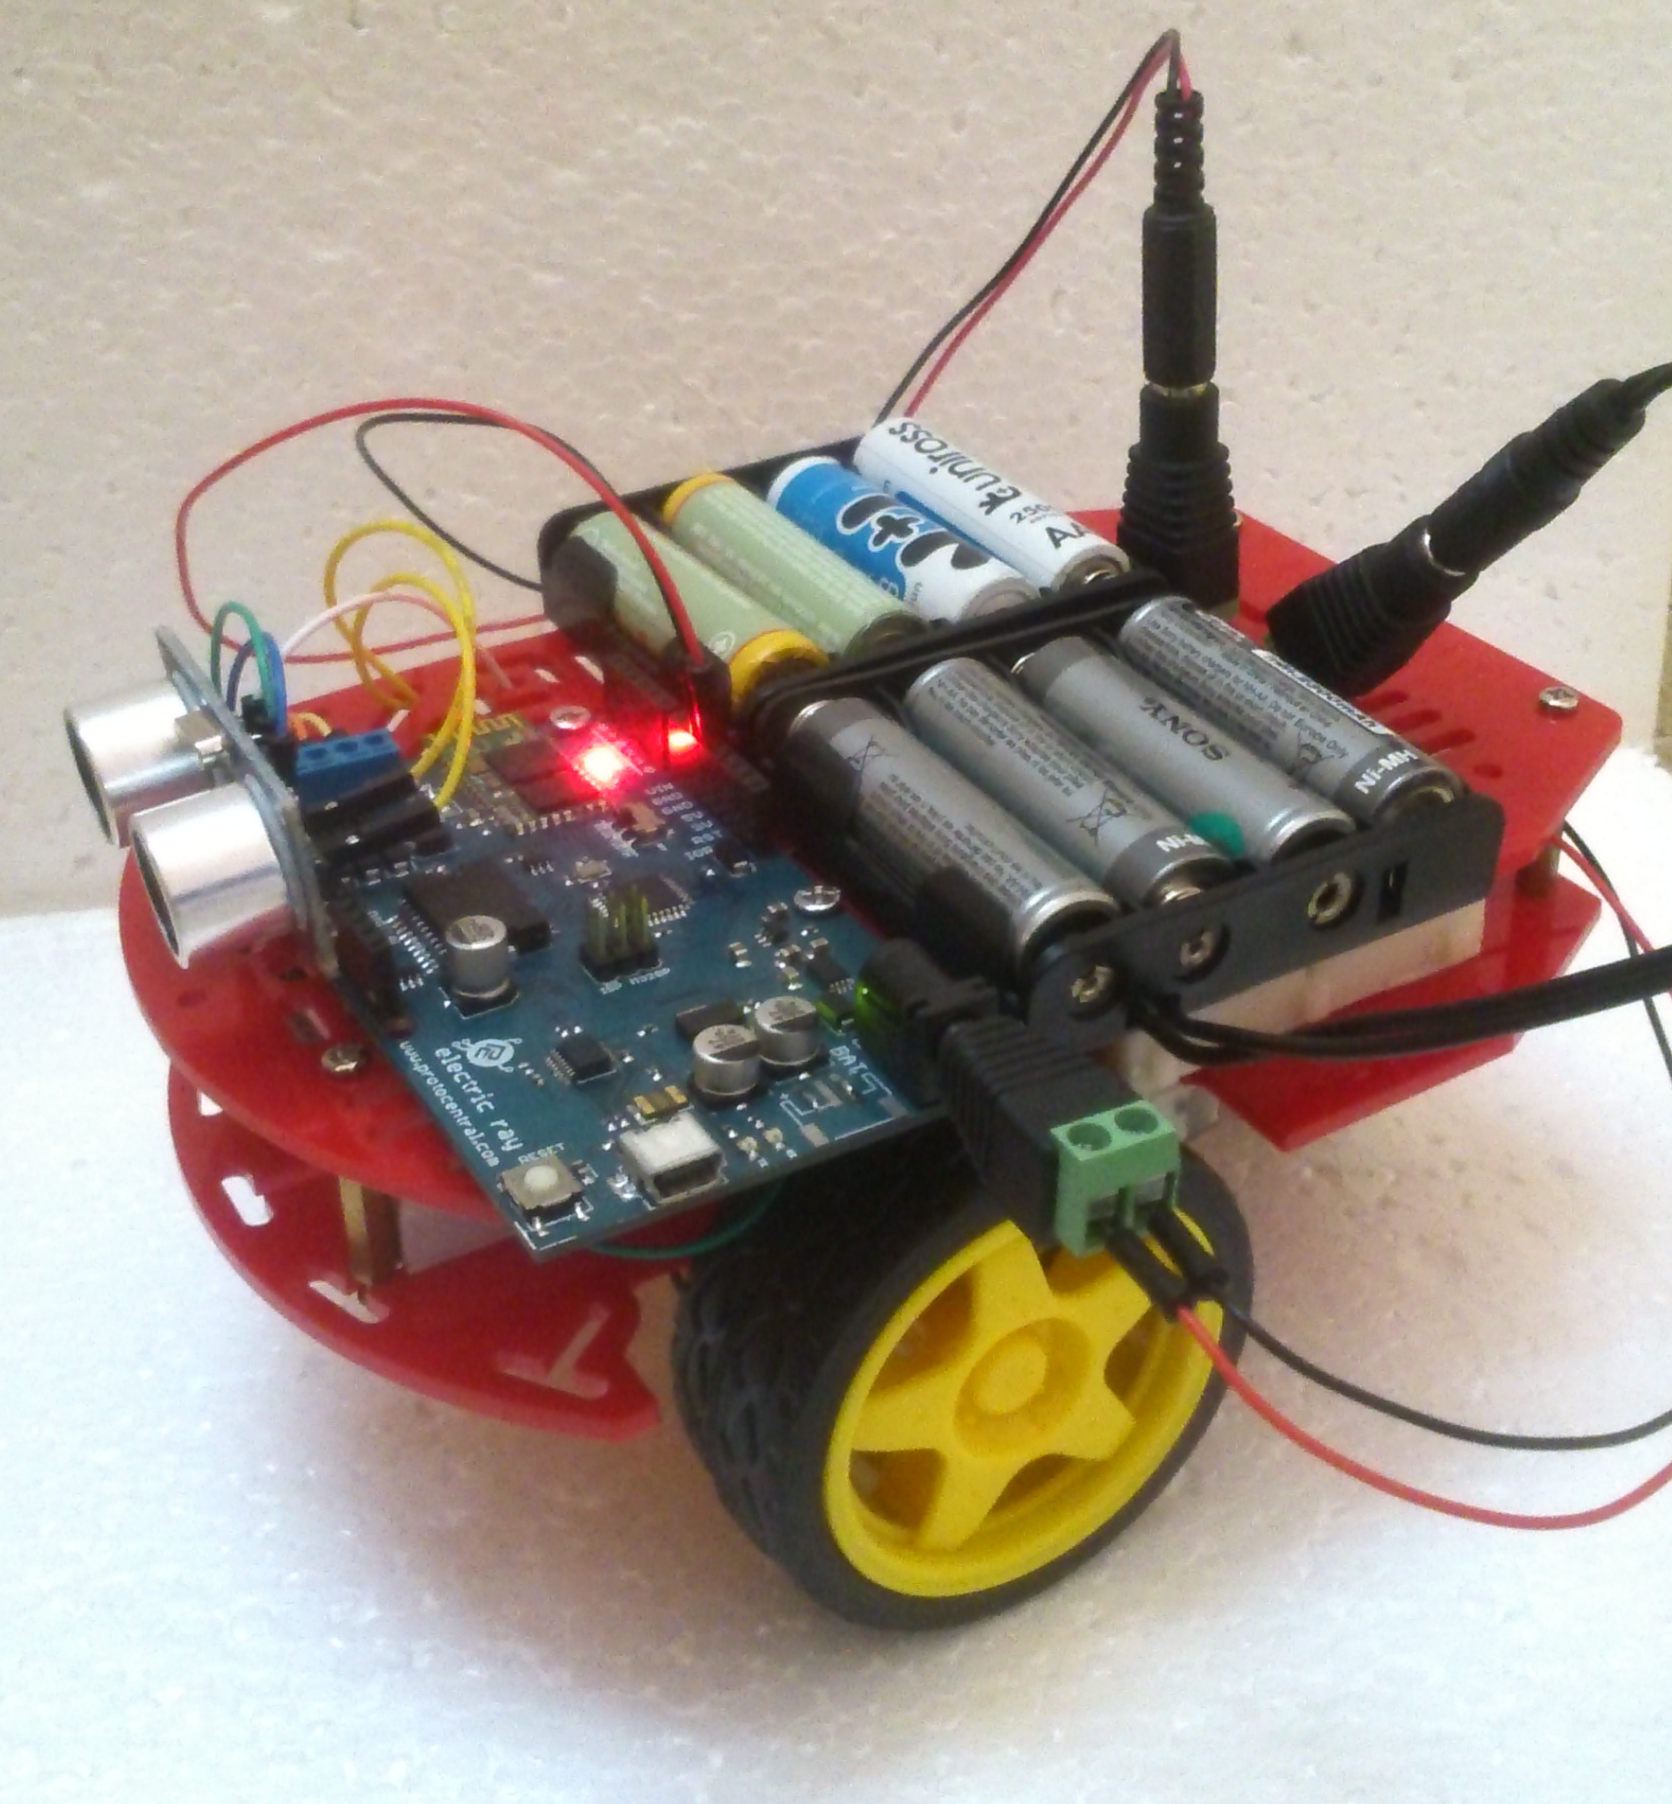
\includegraphics[width=0.4\columnwidth]{Images/InBot}
\caption{InBot}
\label{fig:inbot}
\end{figure}

\section{InBot Hardware}

\begin{figure}[h]
\centering
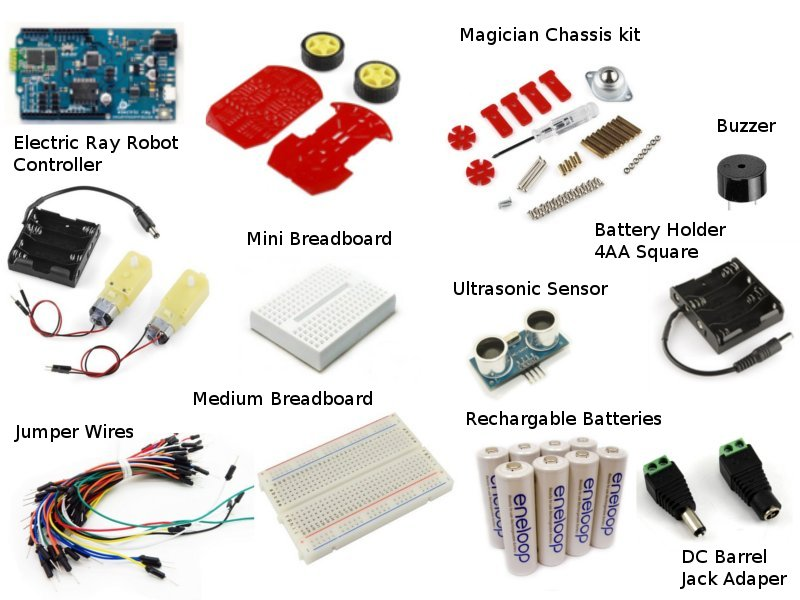
\includegraphics[width=1\columnwidth]{Images/parts}
\caption{InBot hardware components}
\label{fig:components}
\end{figure}

The Magician Chassis is an economical robot platform which features two gearmotors with 65mm wheels and a caster. Electric Ray is a completely integrated, easy-to-use robot controller fully compatible with the Arduino Uno and programmable with the Arduino environment. With an Arduino-compatible Atmega328P microcontroller, dual motor controllers and a Bluetooth module it can be easily assembled to magician chassis.

\begin{table}[!htbp]
\centering
\caption{Component Cost and Vendor details}
\label{tab:cost}
\vspace{2mm}
 \begin{tabular}{||c c c c c ||} 
 \hline
 No & Name & Quantity & Price(Rs.) & Purchased from \\ [0.5ex] 
 \hline\hline
 1 & Magician Chassis kit & 1 & 1150.00 & Tenet Technetronics \\ 
 \hline
 2 & Electric Ray Robot Controller & 1 & 3499.00 & ProtoCentral \\ 
 \hline
 3 & Mini Breadboard (Self Adhesive) & 1 & 89.00 & ProtoCentral \\ 
 \hline
 4 & Medium Breadboard (Self Adhesive) & 1 & 159.00 & ProtoCentral \\ 
 \hline
 %5 & Wheel Encoder & 1 & 949.00 & MG Superlabs India \\ 
 %\hline
 5 & Ultrasonic Sensor & 1 & 99.00 & eBay \\ 
 \hline
 6 & Buzzer & 1 & 75.00 & Tenet Technetronics \\ 
 \hline
 7 & Battery Holder - 4AA Square & 1 & 165.00 & Tenet Technetronics \\ 
 \hline
 8 & DC Barrel Jack Adaper & 2 & 186.00 &  Tenet Technetronics \\ 
 \hline
 9 & Rechargable Batteries & 8 & 849.00 & Amazon \\ 
 \hline
 10 & Jumper Wires ( 65 piece pack) & 1 & 199.00 & ProtoCentral \\ 
 \hline\hline
  & Total &  & 6470.00 &  \\ 
 \hline
\end{tabular}
\end{table}

\section{InBot Assembly}

A step by step illustration of assembling the InBot is shown starting from Figure ~\ref{fig:right_motor}

\begin{figure}[h]
\centering
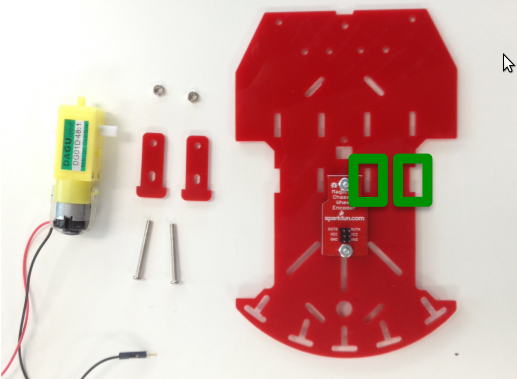
\includegraphics[width=0.4\columnwidth]{Images/Assembly/1a}
\caption{ Before attaching right motor }
\vspace{2mm}
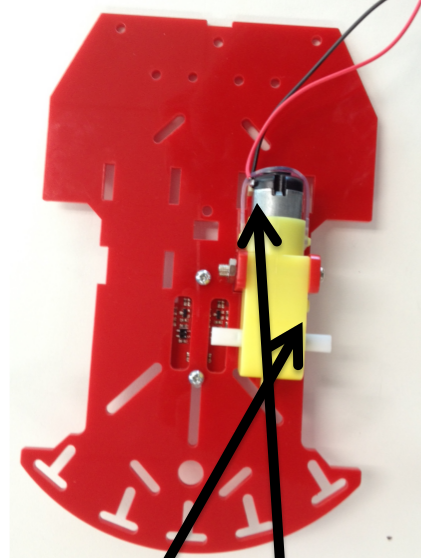
\includegraphics[width=0.4\columnwidth]{Images/Assembly/1b}
\caption{ After attaching right motor }
\label{fig:right_motor}
\end{figure}

\begin{figure}[h]
\centering
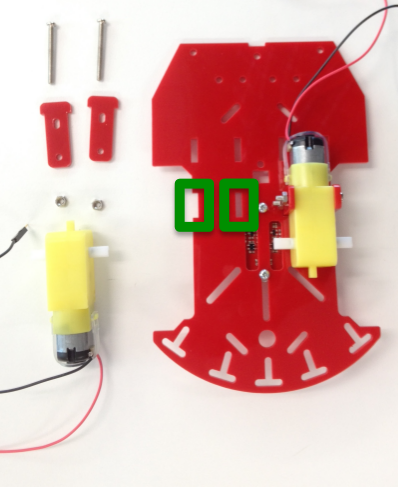
\includegraphics[width=0.4\columnwidth]{Images/Assembly/2a}
\caption{ Before attaching left motor }
\vspace{2mm}
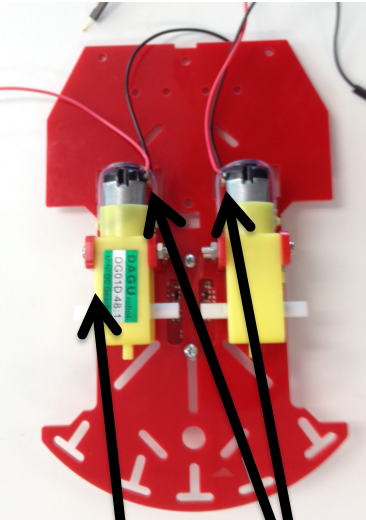
\includegraphics[width=0.4\columnwidth]{Images/Assembly/2b}
\caption{ After attaching left motor }
\label{fig:left_motor}
\end{figure}

\begin{figure}[h]
\centering
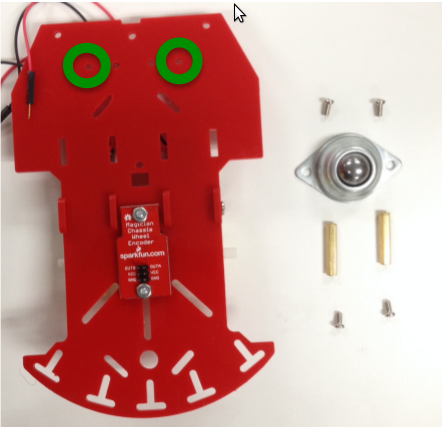
\includegraphics[width=0.4\columnwidth]{Images/Assembly/3a}
\caption{ Before attaching omni wheels }
\vspace{2mm}
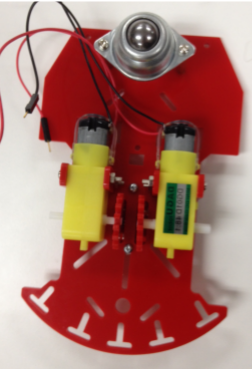
\includegraphics[width=0.4\columnwidth]{Images/Assembly/3b}
\caption{ After attaching omni wheels }
\label{fig:omni_wheels}
\end{figure}

\begin{figure}[h]
\centering
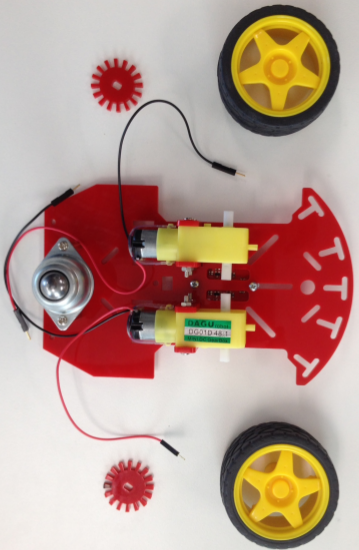
\includegraphics[width=0.4\columnwidth]{Images/Assembly/4a}
\caption{ Before attaching wheels}
\vspace{2mm}
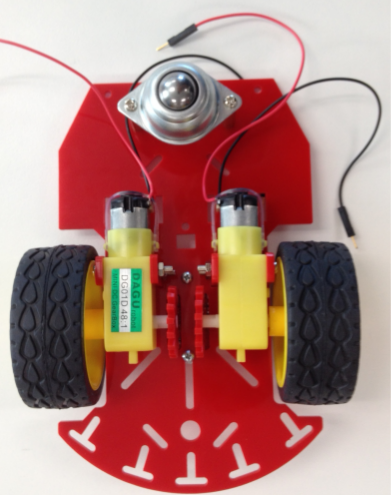
\includegraphics[width=0.4\columnwidth]{Images/Assembly/4b}
\caption{ After attaching wheels}
\label{fig:wheels}
\end{figure}

\begin{figure}[h]
\centering
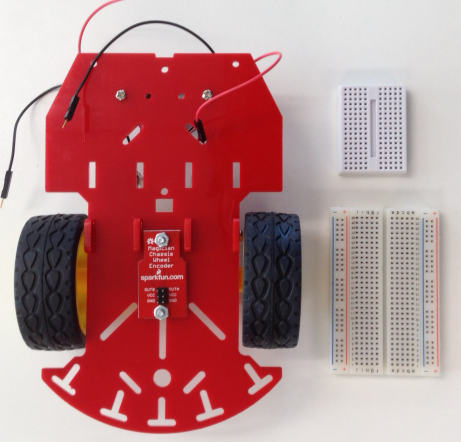
\includegraphics[width=0.4\columnwidth]{Images/Assembly/5a}
\caption{ Before attaching bread boards}
\vspace{2mm}
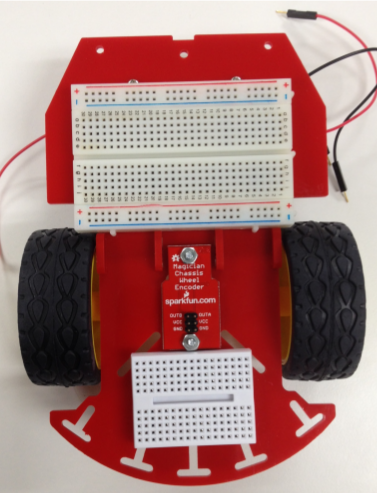
\includegraphics[width=0.4\columnwidth]{Images/Assembly/5b}
\caption{ After attaching bread boards}
\label{fig:boards}
\end{figure}

\begin{figure}[h]
\centering
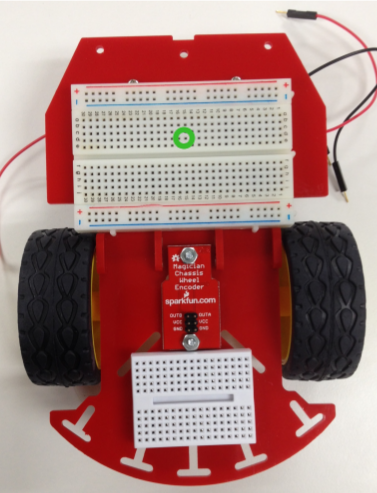
\includegraphics[width=0.4\columnwidth]{Images/Assembly/6a}
\caption{ Before attaching buzzer}
\vspace{2mm}
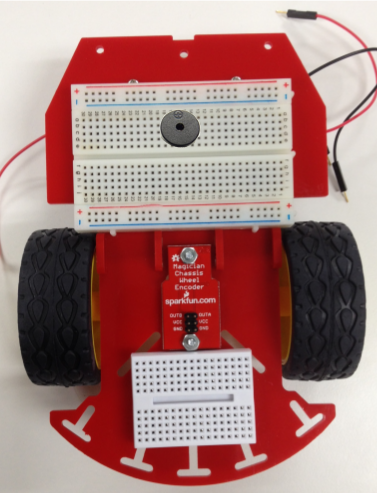
\includegraphics[width=0.4\columnwidth]{Images/Assembly/6b}
\caption{ After attaching buzzer}
\label{fig:buzzer}
\end{figure}

\begin{figure}[h]
\centering
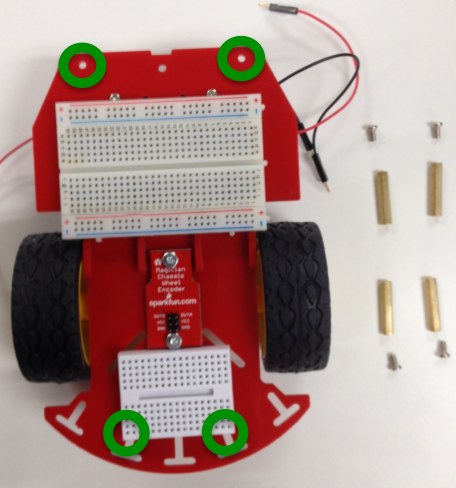
\includegraphics[width=0.4\columnwidth]{Images/Assembly/7a}
\caption{ Before attaching chassis standoffs}
\vspace{2mm}
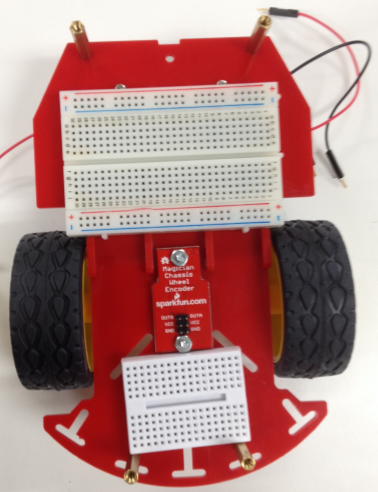
\includegraphics[width=0.4\columnwidth]{Images/Assembly/7b}
\caption{ After attaching chassis standoffs}
\label{fig:buzzer}
\end{figure}
